\chapter{Result}
The focus of my implementation has been to minimize the amount of 
hardware usage, while trying to meet the timing constraints provided 
from the rest of the circuit. The clock frequency used on the FPGA has 
been 100 MHz. A throughput in the scale of Gbits/s is sufficient for the
current design.

The implemented scrambler processes 16 bytes of data in 11 clock pulses 
with a clock frequency of 94MHz, which would correspond 
roughly to a throughput of 1.16 Gbits/s. The scrambler needs to first
process the key, before being able to scramble data. A keyexpansion 
takes roughly 45 clock pulses, and is only performed when a new key is 
sent, which is very seldom. The scrambler then deals with 16 bytes of 
data on 13 clock pulses, but outputs 1 byte of data per clock cycle. 
This is done so that one byte of data from the scrambled package is 
read into a register on every clock pulse. When four bytes are collected
the 32-bit output is sent out. I work with 32-bits, since the data-bus 
is a 32-bit bus.

\section{Problems}
The main problems that I encoutered were:

\begin{itemize}
\item Not possible to get the license for CSA3
\item Small interrest for CSA3
\item Next to no documentation of the CISSA algorithm
\item Hard finding reliable test vectors
\item Merging
\item Timing
\item Latches
\end{itemize}

When I first started writing this Thesis, the thought was that I was to 
implement the CSA3 algorithm. Due to problems with licensing, and the 
fact that AES-128 in CBC-mode seemed like a better idea led to a rework 
of the planning.

Most of these problems are, in my mind, self-explanatory. The one that 
I will discuss here is my problem with merging. This problem occured 
due to the fact that I made a bottoms-up design, instead of the more 
common top-down design. I started the project by implementing small 
entities, that were to be used in higher hierarchies. Doing this caused 
some problems when merging entities into higher level blocks, since 
some signals, which I had not thought about, needed to be produced. 
This was not a huge problem, and only occurred on a few instances, but 
were rather troublesome at those times.

The pro of my method of working has been that I have been able to get 
results quickly. The con is that a large portion of the time has been 
spent on going back to entities that were already functional, and 
reworking them by adding signals, and finding the right timing 
conditions to make sure that they provided nescessary information for 
entities higher up in the hierarchy.

Since I tried to optimize this implementation to just meet the demands 
on speed, while trying to minimize the amount of hardware needed, I 
introduced timing into a few circuits that could have otherwise been 
completely combinatorial. This has, as expected, introduced quite a 
bunch of timing-issues. I dare say that all of them are gone now, but 
it is quite hard to know without testing the circuit more extensively.

When I first synthesized the circuit, towards the end of the 
implementation, I found that the circuit synthesized a large amount of 
latches. This made my circuit take up roughly 15\% of the FPGA, and use 
11830 Flip-Flops (FFs). At this time, there were roughly 3000 latches. 
When I managed to remove all of them, my entire circuit used up roughly 
8\% of the FPGA, and used about 4500 FFs instead.

This is the entire hardware usage, including the interface towards the 
FPGA, which is one of the reasons why it might appear large, when 
compared to other implementations.

\section{Hardware}
The top entity can be viewed in Figure \ref{b:scr}, and the rest of 
the entities can be viewed in appendix \ref{app:blocks}.

\begin{figure}
  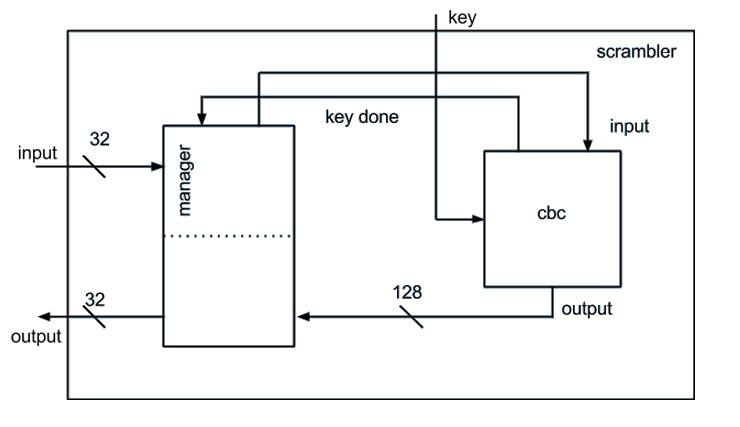
\includegraphics[width=\textwidth]{scrambler}
  \caption{The top entity}
  \label{b:scr}
\end{figure}

\subsection{Hardware usage}
REWRITE WO SHITE

%% I have run five rounds of synthesis on my circuit. The first two ones 
%% were performed on the entire scrambler, including the manager 
%% (interface towards the rest of the FPGA), while the last synthesis were 
%% performed on each block of the circuit seperately.

\subsubsection{First synthesis}
The circuit used up 15\% of the FPGA, and had quite a large amount of 
unnescessary latches and FFs included. It used 11830 FFs, and roughly 
3000 latches. I redesigned the circuit to remove the latches and ran 
the second synthesis.

\subsubsection{Second synthesis}
The circuit used up 8\% of the FPGA this time. The keyblock3 entity, as 
well as keyblock1 entity seemed to use a lot of registers and 
multiplexers, which could possibly be replaced by RAMs or LUTs.

The maximum frequency obtained was 92MHz after this synthesis. This 
was largely due to routing, which made up for 75\% of the minimum 
period.

To be able to compare the third synthesis with this one, you need to 
know that the keyexpansion entity used 1538 D-type FFs and 16 
Comparators. It used up 176 8-bit registers, which were used by the 
expanded key.

\subsubsection{Third synthesis}
Before running this synthesis, I noticed that at one point the circuit 
waited for the expanded key to become done before outputting it. While 
this is a good idea, no problems were noticed I assigned the expanded 
key while it was being updated. Therefore I managed to theoretically 
cut down the hardware by 176 8-bit registers, which should corespond to 
roughly 1408 D-type FFs. 

The vector that was removed was a vector containing 11 * 16 bytes of 
data, which corresponds to 176 * 8 bits of data. 176 times 8 is 1408, 
which is the number of D-type FFs needed to store the value, which 
also corresponds to 176 8-bit registers.

The entire circuit still used up roughly 8\% of the FPGA. The 
keyexpansion entity used 130 D-type FFs and 16 Comparators this 
time. This corresponds to a decrease of 1408 D-type FFs.

The maximum frequency obtained this time was 94MHz. The number of 
Slice Registers went down from 4357 to 2945, and the percentage of 
Slice Registers decreased from 3\% usage to 2\% usage.

The keyblock3 module seems to be using the most hardware from what can 
be seen. It uses roughly 1302 multiplexers, which should be reducable.

\subsubsection{Fourth synthesis}
The next synthesis was made after the state2data module was rewritten, 
to remove yet another signal. This should have decreased the design by 
a 128-bit register. It was mostly done to try to allow for a synthesis 
of the module, while also reducing hardware usage. This should decrease 
the number of D-type FFs by yet another 128. A comparison between 
report 3 and 4 displays a decrease from 130 D-type FFs to 2 D-type FFs.

The maximum frequency obtained this time was 94MHz. The number of 
Flip-Flops went from 2945 to 2817. This did not affect the number of 
Slice Registers.

The circuit still uses roughly 8\% of the hardware on the FPGA.

\subsubsection{Fifth synthesis}
When I got about to this point of synthesis and optimization I found 
that two files were created during each synthesis. A Synthesis Report 
as well as a Place and Route Report. The ones I have been taking a look 
at this far have been the Synthesis Reports, and to make sure that 
there are not any huge gaps in numbers between the reports, I will 
continue to read them, and not the Place and Route Reports. Many of the 
entities can not be mapped seperately, due to the amount of IOs on the 
FPGA, compared to the number of IOs required by the modules.

The third synthesis was performed on each block seperately, to find out
where optimization might be performed. The usage can be viewed in Table 
\ref{synt:fifth}.

%
\newcommand{\MyIndent}{\hspace*{0.2cm}}%

\begin{longtable}{ l | c | c }
  Entity & Slice LUTs out of 63288 & Slice Registers out of 
  126576 \\ \hline
  scrambler              & 5167 & 2817 \\
  \MyIndent \triangleright manager      &  858 &  699 \\ 
  \MyIndent \triangleright cbc          & 4321 & 2127 \\

  \MyIndent \MyIndent \triangleright cipher       & 4229 & 1994 \\

  \MyIndent \MyIndent \MyIndent \triangleright keyexpansion & 2914 
  & 1601 \\

  \MyIndent \MyIndent \MyIndent \MyIndent \triangleright keyblock1 
  & 689 & 0 \\
  \MyIndent \MyIndent \MyIndent \MyIndent \triangleright keyblock2 
  & 208 & 9 \\

  \MyIndent \MyIndent \MyIndent \MyIndent \MyIndent \triangleright 
  demux & 32   & 0 \\
  \MyIndent \MyIndent \MyIndent \MyIndent \MyIndent \triangleright 
  keycore & 183 & 9 \\

  \MyIndent \MyIndent \MyIndent \MyIndent \MyIndent \MyIndent 
  \triangleright ctr & 14 & 9 \\
  \MyIndent \MyIndent \MyIndent \MyIndent \MyIndent \MyIndent 
  \triangleright rotw & 0 & 0 \\
  \MyIndent \MyIndent \MyIndent \MyIndent \MyIndent \MyIndent 
  \triangleright sbox & 128 & 0 \\
  \MyIndent \MyIndent \MyIndent \MyIndent \MyIndent \MyIndent 
  \triangleright rcon & 40 & 0 \\

  \MyIndent \MyIndent \MyIndent \MyIndent \triangleright keyblock3 
  & 1854 & 1365 \\

  \MyIndent \MyIndent \MyIndent \triangleright data2state & 0 
  & 0 \\
  \MyIndent \MyIndent \MyIndent \triangleright round & 1535 & 272 \\

  \MyIndent \MyIndent \MyIndent \MyIndent \triangleright subbytes 
  & 512 & 0 \\
  \MyIndent \MyIndent \MyIndent \MyIndent \triangleright shiftrows 
  & 0 & 0 \\
  \MyIndent \MyIndent \MyIndent \MyIndent \triangleright mixcolumns 
  & 176 & 0 \\
  \MyIndent \MyIndent \MyIndent \MyIndent \triangleright addkey & 128 
  & 0 \\

  \MyIndent \MyIndent \MyIndent \triangleright state2data & 1 & 2 \\

  \caption{Hardware usage of entities}
  \label{synt:fifth}
\end{longtable}

My plan was to try to reduce the critical path by inserting FFs in the 
middle of it and then run another synthesis. This would have increased 
the hardware by a lot of FFs, but also increased the maximum frequency. 
This was hard to do due to timing issues, which is why I decided to 
change the UCF instead of spending the time trying to decrease the 
critical path, only to increase the amount of hardware.

Running this synthesis let me know that you are not informed whether the
desired frequency can be achieved or not, when you run the synthesis 
using an UCF. Because of this, I once again tried to add the FFs to 
shorten the cricical path. 

\subsubsection{Sixth synthesis}
The final synthesis I ran on the circuit gave the following results:

\section{Further development}
There are, as usual, an amount of optimization that could be performed 
on the circuit. They consist of optimization of code, as well as some 
deeper research into how to rewrite VHDL code to turn the registers in 
this implementation into RAMs, ROMs or LUTs.

\subsection{Rijndael's S-Box}
The Rijndael Sbox implemented in my design does not synthesize into a 
ROM, which it should be able to do. Other than a ROM, it should also be 
able to be synthesized into a couple of LUT6.
I have not been able to find out why my code is implemented into 
registers instead of more efficient solutions, but it is. 

\subsection{Critical Path}
To increase the maximum frequency of the circuit, the critical path 
needs to be decreased. This is done by adding FFs in the middle of the 
critical path. This will be hard to solve, due to the complexity of the 
keyexpansion, and would increase the amount of hardware as well as the 
complexity of the circuit if FFs were to be added.

The decision whether to reduce the critical path, or not, is a hard 
decision due to the vast amount of hardware that needs to be added to
increase the frequency.
%% \subsection{HARDUNÅGOTMERDUVILLFÖRBÄTTRA?}

\section{Implementation}
My design is very hierarchical. The top layer is an aes128 block in 
CBC-mode. It takes an input TS-packet, selects data from it which it 
scrambles, and then outputs the data in the form of a TS-packet once 
again.

The scrambler consists of two entities. An entity which I call the 
cbc-entity, which deals with the scrambling of the received data. The 
other entity is a data-manager. The manager deals with reading data 
from the interface towards the rest of the FPGA as well as sending the 
right data-bits to the CBC-entity. It also tells the CBC-entity how to 
handle the data, since different things are to be done depending on if 
the data is the first data packet sent, or not.

\subsection{Manager entity}
The manager (Figure \ref{block:manager}) consists of a FIFO, an FSM and 
a couple of registers. The FIFO is needed since the data sent to the 
scrambler from the FPGA is sent in bursts. The FIFO therefore writes 
the data bursts into a memory, from which it later reads, processes and 
sends the data to the CBC-entity. The data written to the FIFO is 
written in packets of 32 bits, but are read 8 bits at the time. The 
manager looks through the data packets to see if there is an adaptation 
field or not, since that changes the way we handle the data. The 
payload is written to the first set of registers as the data is found, 
and then sent to the next set of registers. This is simply done to 
allow the manager to deal with two sets of data in parallell. When the 
packet is ready to be sent, a flag is set and the data is sent to the 
CBC-entity. 

\subsection{CBC entity}
The CBC-entity (Figure \ref{block:cbc}) consists of three small 
entities. An XOR, a multiplexer and a cipher-entity. The multiplexer is 
needed since we want to input the first plaintext into the XOR together 
with an IV. We want to use the output ciphertext instead of the IV for 
the rest of the plaintexts contained within the same TS-packet. There 
is only going to be one aes128 cipher in the CBC-entity, in order to 
save hardware. It will be run in sequence instead of in parallell, even 
though it might reduce the maximal speed of the circuit.

\subsection{Cipher entity}
The aes-128 cipher-entity (Figure \ref{block:cipher}) consists of 4 
components. The data2state entity, which transforms the array into a 
matrix of data. A keyexpansion entity, which takes an input of a key, 
and generates an extended key as an output. An entity, which I chose to 
call rounds, which deals with the encryption of the 16 byte blocks. And 
finally a state2data entity, which transforms the data-matrix into an 
array once again. The cipher entity itself keeps track of timing mainly 
between the keyexpansion and the round entity, and makes sure to 
provide the round entity with the correct roundkey at the right time.

\subsection{Keyexpansion entity}
The keyexpansion-entity is divided into 3 keyblock entities. The first 
keyblock entity decides what 4 bytes of the expanded key we want to 
expand. The second keyblock entity contains the keycore, which is only 
performed on every 4th set of 4 bytes, and a demux entity. The third 
keyblock entity performs an xor and an incrementation of the internal 
counter used as an index when accessing 4 byte blocks of data.

\subsubsection{Keycore entity}
The keycore entity consists of four entities. Rotword, Sbox, Rcon and a 
counter. The counter is used to get the right data-byte from the Rcon 
entity, and the index is only used in the keycore, and is thus best 
suited to be placed inside the keycore entity. Rotword rotates the 
bytes of the input one step to the left. Sbox replaces the input bytes 
according to the Rijndael Sbox. The Rcon entity both collects the 
correct rcon value from a precalculated vector, as well as inputs it 
into an xor together with the input.

\subsection{Round entity}
The round-entity (Figure \ref{block:round}) consists of four entities. 
Subbytes, shiftrows, mixcolumns and addroundkey. Addroundkey is a 
somewhat special XOR. Subbytes is an Rijndael Sbox, which takes an 
input 16-byte state, substitutes it, and outputs another 16-byte state. 
Shiftrows transposes the rows of the second, third and fourth row of 
the state. Last, but not least, is the mixcolumns entity. It consists 
of 16 mulblock entities. The input state of mixcolumns is split into 
columns, and each column is sent to a mulblock entity, which multiplies 
the inputs with 1, 2 or 3, then performs a bitwise XOR on them, 
outputting the result of the XOR. The function of the mixcolumns block 
is a rather complex matrix multiplication.

\subsubsection{Addroundkey entity}
Addroundkey is an entity which takes different inputs depending on 
what round we are currently dealing with. On the first round, 
addroundkey takes the input to the round entity. On the last round, it 
takes the output from the subbytes entity. The input to addroundkey is 
the output from mixcolumns the rest of the time.

\subsubsection{The mulblock entity}
The mulblock entity consists of one mul3 entity and one mul2 entity, 
which performs a special kind of hardware multiplication of 3, and 2, 
on the input. It also takes two inputs which it leaves alone. The four 
results are then XOR:ed with eachother, and returned to the mixcolumns 
entity. The result is then input into the correct index in the matrix. 

Mul3 means multiplication with 3, and mul2 means multiplication with 2. 
A multiplication with 2 is a left-shift, followed by an XOR with the 
fix value 0x1B if the shifted value exceeds 0xFF. A multiplication with 
3 is the same as a multiplication with 2, followed by an XOR with the 
input value.

\section{Tests}
All of the entities in the design have been simulated and evaluated 
seperately before being merged and tested together, to make sure that 
they had the desired functionality both seperately and when combined 
together. The simulations for the seperate blocks are trivial, and 
therefore not included in the report.

Figure \ref{test:1} through \ref{test:3} are tests performed on the 
complete aes-128 block, before CBC-mode. In the figures, in\_key is the 
input key to be extended and used, and datapacket is one packet from a 
TS. Test vector 1 and 2 are taken from \citep{AES:2001}, while test 
vector 3 is generated using a webpage.

\emph{Test vector 1 (Figure \ref{test:1})}\\
Input key: 2b 7e 15 16 28 ae d2 a6 ab f7 15 88 09 cf 4f 3c\\
Plaintext: 32 43 f6 a8 88 5a 30 8d 31 31 98 a2 e0 37 07 34\\
Ciphertext: 39 25 84 1d 02 dc 09 fb dc 11 85 97 19 6a 0b 32

\begin{figure}
  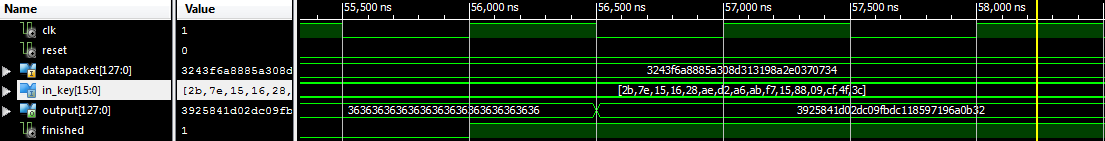
\includegraphics[width=\textwidth]{successtv1}
  \caption{Test vector 1}
  \label{test:1}
\end{figure}

\emph{Test vector 2 (Figure \ref{test:2})}\\
Input key: 00 01 02 03 04 05 06 07 08 09 0a 0b 0c 0d 0e 0f\\
Plaintext: 00 11 22 33 44 55 66 77 88 99 aa bb cc dd ee ff\\
Ciphertext: 69 c4 e0 d8 6a 7b 04 30 d8 cd b7 80 70 b4 c5 5a

\begin{figure}
  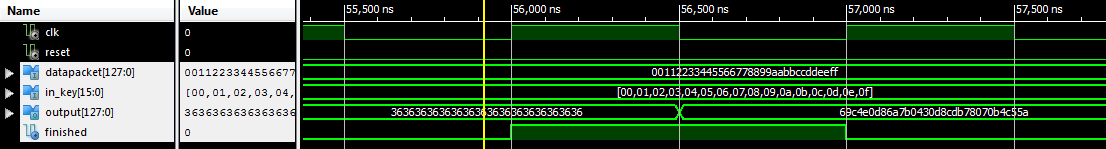
\includegraphics[width=\textwidth]{successtv2}
  \caption{Test vector 2}
  \label{test:2}
\end{figure}

\emph{Test vector 3 (Figure \ref{test:3})} \\
Input key: 10 20 30 40 50 60 70 80 90 a0 b0 c0 d0 e0 f0 bb\\
Plaintext: 00 11 22 33 44 55 66 77 88 99 aa bb cc dd ee ff\\
Ciphertext: bf 99 1f aa 8b 0f e6 48 36 46 a0 2d 33 9e de a5

\begin{figure}
  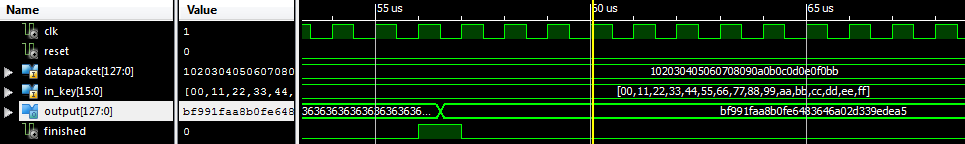
\includegraphics[width=\textwidth]{successtv3}
  \caption{Test vector 3}
  \label{test:3}
\end{figure}

\section{Discussion}
The main reason for choosing a bottoms-up methodology, was since the 
functionality of the smaller blocks were very basic, but the timing was 
rather complex. In addition to the fact that there were no concrete 
guidlines, performing the work on the smaller entities, and then 
implementing the higher ones minimized the probability of performing 
tasks that were to be discarded in later stages of the implementation.

\section{Conclusions}
One of the first things I learned during this thesis was that industrial
secrecy can put a quick halt to projects. A license had to be written 
and approved by ETSI before WISI Norden was allowed information about 
the specifications of one of the algorithms that I was supposed to 
analyze. Due to restrictions, this could not be done, meaning that 
this specific analyzis came to a halt before it even started. This 
led to the comparison between a software- and hardware-friendly 
algorithm becoming impossible to do. 

While WISI Norden and ETSI were discussing the license, I tried to find 
out specifics about the CSA3 and CISSA algorithm, since those were the 
ones that I was to analyze. From the little information available about 
the CSA3, only the names of the two ciphers were possible to find. 
Since one of the two ciphers in the CSA3 algorithm corresponded to one 
of the ciphers in the CISSA algorithm, I decided to look into this 
cipher as much as possible. This was the AES-128 cipher.

Both the key generation, and the functionality of the entities in 
AES-128 algorithm could be found in litterature, since the AES 
encryption is a public algorithm. From what I could find out about 
the CISSA algorithm, through an official ETSI journal, it seemed to 
just use the AES-128 algorithm, but in a certain mode, with a specific 
Initialization Vector. This 
